% TEMPLATE for Usenix papers, specifically to meet requirements of
%  USENIX '05
% originally a template for producing IEEE-format articles using LaTeX.
%   written by Matthew Ward, CS Department, Worcester Polytechnic Institute.
% adapted by David Beazley for his excellent SWIG paper in Proceedings,
%   Tcl 96
% turned into a smartass generic template by De Clarke, with thanks to
%   both the above pioneers
% use at your own risk.  Complaints to /dev/null.
% make it two column with no page numbering, default is 10 point
% Munged by Fred Douglis <douglis@research.att.com> 10/97 to separate
% the .sty file from the LaTeX source template, so that people can
% more easily include the .sty file into an existing document.  Also
% changed to more closely follow the style guidelines as represented
% by the Word sample file.
% Note that since 2010, USENIX does not require endnotes. If you want
% foot of page notes, don't include the endnotes package in the
% usepackage command, below.
% This version uses the latex2e styles, not the very ancient 2.09 stuff.
\documentclass[letterpaper,10pt]{article}
%\usepackage{usenix,epsfig,endnotes}
\usepackage{fullpage,epsfig,endnotes,mathtools}
\begin{document}
%make title bold and 14 pt font (Latex default is non-bold, 16 pt}

\title{\Large \bf 18-545: OpenGL Graphics Acelerator}
%for single author (just remove % characters)
\author{
{\rm Andrew J.\ Lau, Alan X.\ Zhu, and Nathan L.\ Wan}\\
\{ajlau, axz, nlw\}@andrew.cmu.edu\\
Carnegie Mellon University
% copy the following lines to add more authors
% \and
% {\rm Name}\\
%Name Institution
} % end author

\date{December 8, 2010}

\maketitle
\newpage
\tableofcontents
\listoffigures
\listoftables
\newpage
% Use the following at camera-ready time to suppress page numbers.
% Comment it out when you first submit the paper for review.
\thispagestyle{empty}

\section{Introduction}
This report discusses an OpenGL graphics accelerator implemented on a Xilinx XUPV5-LX110T FPGA during the Fall 2010 iteration of the Advanced Digital Design capstone course at Carnegie Mellon University. We cover the overall system design, implementation details, and advice for adding further functionality to the system in the future.

\section{System Overview}
The graphics accelerator can be broken down into five major components:
\begin{enumerate}

\item Perl Parser

\item Instruction Assembler

\item Instruction Cache

\item Coordinate Transformation Pipeline

\item Rasterization Unit

\item Framebuffer/Display

\end{enumerate}
<insert system diagram here>

\section{System Specification}
\subsection{Hardware}
\begin{itemize}

\item Microblaze processor

\item Floating point units

\item Coordinate Transformation Pipeline

\item Rasterization Unit

\item Instruction Cache

\item FIFOs

\item Framebuffer Controller

\end{itemize}

\subsection{Software}
\begin{itemize}

\item Perl Parser

\item Instruction Assembler (running on Microblaze)

\end{itemize}

\subsection{Development Software}
\begin{itemize}

\item Xilinx ISE Design Suite 12.2

\item Git

\item Windows XP

\item Ubuntu

\end{itemize}

\section{OpenGL}
\subsection{Rationale}
We chose to implement an OpenGL pipeline because it is a well known industry standard for 2D/3D graphics. In addition, the pipeline design itself is well documented with numerous existing implementations in both hardware and software. When deciding on the project, an OpenGL pipeline seemed appropriate in scope and difficulty for a semester-long undergraduate course.

\subsection{Supported Functions}

The pipeline supports the following subset of OpenGL calls:
\begin{verbatim}
	glBegin (void)
	glEnd (void)
	glVertex (float x, float y, float z)
	glColor (float r, float g, float b)
	glFlush (void)
	glMatrixMode (enum mode)
	glMultMatrix (const float *m)
	glLoadMatrix (const float *m)
	glPushMatrix (void)
	glPopMatrix (void)
	glRotate (float angle, float x, float y, float z)
	glScale (float x, float y, float z)
	glTranslate (float x, float y, float z)
	glViewport (int x, int y, int width, int height)
	glFrustum (int left, int right, int bottom, int top, int near, int far)
	glOrtho (int left, int right, int bottom, int top, int near, int far)
\end{verbatim}

\subsection{Interface to Pipeline}

\subsubsection{Perl Parser}
In order for the pipeline to accept graphical language calls, a Perl script was written that takes human readable trace of OpenGL calls and outputs a hex representation of the program. \\

The trace is generated from simple hand-generated C programs. Conditionals, loops, and variables are unrolled and substituted so that what remains is strictly OpenGL calls and data in the form of actual numeric values. These traces correspond to the calls that would be made by a C library such as GLSim.\\

The main function of the script is to parse each GL call, generate a 32-bit hex value that corresponds to the instruction code defined in the ISA, and output the hex value to a file. If there are argument parameters in the call, each parameter is translated into its hex representation and printed on subsequent lines in the file. The output is an OPNGG hex file (*.gg). Each line of the file is one hex value, either corresponding to an instruction call or one of several 32-bit arguments encoded in hex (single precision floating point , unsigned integer, etc.)

\subsubsection{Instruction Assembler}
The Microblaze processor is critical for programming the accelerator.  To program the instruction cache, the Microblaze reads off a file containing the graphical program and copies in data.  The file resides on the Compact Flash and its format guaranteed by the Perl Parser; the assembler does not check the format of the executable.  The SDK's XilFATFS is a library that allows the Microblaze to read files on the Compact Flash.  For the most part, it follows the C convention for file handling.  The instruction BRAM has an interface identical to that of the Xilinx BRAM cores.  This is so that a PLB to BRAM interface core, provided by Xilinx, can be used to allow the Microblaze to write directly into the instruction cache.  


\section{Instruction Set Architecture}

\subsection{Specification}

The ISA defines a 32-bit instruction word to align with the width of single precision floating point word. The \emph{opcode} field is 8 bits wide, allowing support for up to 256 different routines. This is leaves plenty for room for extending the pipeline to support other some of the 300+ OpenGL calls, as only 17 slots are filled in the current state. The fetch unit addresses the instruction cache at a 32-bit granularity.

\begin{table}[h]
\begin{center}
\begin{tabular}{ | l | l | l | l |}
\hline
Bits & [31] & [30:8] & [7:0] \\ \hline
Content & \emph{type} & \emph{data} & \emph{opcode} \\ \hline
\end{tabular}
\end{center}
\caption{Instruction word}
\end{table}

Each supported function is translated by the Perl parser into the follow instruction words. The \emph{data} field indicates to the fetch unit to expect a certain number of floats following the instruction word if the \emph{type} field is set.

\begin{table}[h!]
\begin{center}
\begin{tabular}{ | l | l | l | l |}
\hline
Function & Type & Data & Opcode \\ \hline
\verb!glBegin (void)! & 0 & X & 00000001 \\ \hline
\verb!glEnd (void)! & 0 & X & 00000010 \\ \hline
\verb!glVertex (float x, float y, float z)! & 1 & 3 & 00000011 \\ \hline
\verb!glColor (float r, float g, float b)! & 1 & 3 & 00000100 \\ \hline
\verb!glFlush (void)! & 0 & X & 00000101 \\ \hline
\verb!glMatrixMode (enum mode)! & 0 & imm & 00010000 \\ \hline
\verb!glMultMatrix (const float *m)! & 0 & 16 & 00010001 \\ \hline
\verb!glLoadIdentity (void)! & 0 & X & 00010010 \\ \hline
\verb!glLoadMatrix (const float *m)! & 1 & 16 & 00010011 \\ \hline
\verb!glPushMatrix (void)! & 0 & X & 00010100 \\ \hline
\verb!glPopMatrix (void)! & 0 & X & 00010101 \\ \hline
\verb!glRotate (float angle, float x, float y, float z)! & 1 & 4 & 00010110 \\ \hline
\verb!glScale (float x, float y, float z)! & 1 & 3 & 00010111 \\ \hline
\verb!glTranslate (float x, float y, float z)! & 1 & 3 & 00011000 \\ \hline
\verb!glViewport (int x, int y, int width, int height)! & 1 & 4 & 00011001 \\ \hline
\verb!glFrustum (int left, int right, int bottom, int top, int near, int far)! & 1 & 6 & 00011010 \\ \hline
\verb!glOrtho (int left, int right, int bottom, int top, int near, int far)! & 1 & 6 & 00011011 \\ \hline
\end{tabular}
\end{center}
\caption{OpenGL routine to opcode mappings}
\end{table}

\section{Fetch and Decode}
\subsection{Instruction Cache}
The instruction cache consists of 512 entries of 32-bit words and supports 5 reads and 1 write - concurrently serving the fetch, decode, and instruction assembler through a BRAM controller on the PLB. It is currently implemented in logic, with a combinational read. Further work would be needed to move the instruction cache into block RAM, requiring a clocked read.

\subsection{Fetch Unit}
The fetch unit reads one 32-bit word per cycle from the instruction cache, stalling if the vertex and color FIFOs are full and during matrix operations.

\subsection{Decode Unit}
The decode unit generates control signals for the matrix stacks, matrix multipliers, perspective division, and viewport transformation. It also reads 4 32-bit words from the instruction cache for use in the latter pipeline stages.

\section{Matrix Operations}

\subsection{Matrix Stacks}
The pipeline implements two 16x16 matrix stacks - one for Modelview matrices, one for Projection matrices. The bottom of each stack is initialized to the identity matrix by default, with the stack pointer initialized to point at the bottom. The matrix stacks are currently implemented in logic to support combinational reads, but could be moved to BRAM fairly easily. 

\subsection{Matrix Multiply}
Since the coordinate transformation takes relatively short amount of time when compared to the rasterizer, the decision was made to utilize less floating point units and allow a matrix multiply to take 4 cycles per row, or 16 cycles for a 4x4 x 4x4 multiply. Matrices are updated 1 row at a time, with a row update module that utilizes 4 floating point multipliers and 3 floating point adders. The fetch unit is stalled while a matrix multiply occurs, since most of the supported functions utilize the matrix stacks. Because each vertex is multiplied by both the Modelview and Projection matrices, this means that each call to \verb!glVertex! takes 32 cycles on the coordinate transform clock.



\section{Coordinate Transformation}
Each vertex (consisting of 3 floating point numbers corresponding to x, y, z coordinates) that gets passed into Coordinate Transformation goes through a series of transformations so that it ends up in the correct range to be displayed on the screen. The resulting vertices and their corresponding colors are pushed into a dual clocked FIFO.

\subsection{Eye Coordinates}
The incoming vertex is multiplied by the modelview matrix to produce \emph{eye coordinates}. The modelview matrix is a the combination of the model and view matrices. Since there is no separate camera in OpenGL, the scene must be transformed by the inverse of the view transformation to simulate moving the camera.\\

\begin{figure}[h]
\[
\begin{pmatrix}
x_{eye} \\
y_{eye} \\
z_{eye} \\
w_{eye}
\end{pmatrix}
= M_{modelview} \cdot
\begin{pmatrix}
x_{obj} \\
y_{obj} \\
z_{obj} \\
w_{obj}
\end{pmatrix}
\]
\caption{Eye Coordinates}
\end{figure}

\subsection{Clip Coordinates}
The eye coordinates are multiplied by the projection matrix to produce clip coordinates, in which objects that are not in the viewing frustum are clipped out. The viewing frustum is set by calls to \verb!glFrustum! and \verb!glOrtho! for perspective and orthographic projection, respectively. \\
\begin{figure}[h]
\[
\begin{pmatrix}
x_{clip} \\
y_{clip} \\
z_{clip} \\
w_{clip}
\end{pmatrix}
= M_{projection} \cdot
\begin{pmatrix}
x_{eye} \\
y_{eye} \\
z_{eye} \\
w_{eye}
\end{pmatrix}
\]
\caption{Clip Coordinates}
\end{figure}

\subsection{Perspective Division}
Perspective division yields coordinates known as \emph{normalized device coordinates}, with their range normalized to $(-1,1)$ for all 3 axes.\\
\begin{figure}[h]
\[
\begin{pmatrix}
x_{ndc} \\
y_{ndc} \\
z_{ndc}
\end{pmatrix}
=
\begin{pmatrix}
x_{clip}/w_{clip} \\
y_{clip}/w_{clip} \\
z_{clip}/w_{clip}
\end{pmatrix}
\]
\caption{Perspective Division}
\end{figure}

\subsection{Viewport Transformation}
Viewport transformation scales and translates the normalized device coordinates to fit the rendering screen. The results $(x_{w},y_{w},z_{w})$ are passed to the rasterizer. The transformation is given by: \\
\begin{figure}[h!]
\[
\begin{pmatrix}
x_{w} \\
y_{w} \\
z_{w}
\end{pmatrix}
=
\begin{pmatrix}
\frac{w}{2}x_{ndc}+(x+\frac{w}{2}) \\
\frac{h}{2}y_{ndc}+(y+\frac{h}{2})  \\
\frac{f-n}{2}z_{ndc}+\frac{f+n}{2}
\end{pmatrix}
\]
\caption{Viewport Transformation}
\end{figure}\\	
With some factoring, this is implemented using three floating point multipliers and five floating point adders.


\section{Rasterization}

The purpose of rasterization is to take sets of vertices from coordinate transform, and figure out which pixels on the screen should be drawn which color so that the correct primitive gets displayed on the screen in the correct position. 

In our project, we dealt only with triangles. This means the rasterizer would dequeue sets of 3 vertices from both the vertex FIFO and color FIFO that the coordinate transform pipeline fills. Each vertex dequeued from the vertex FIFO is a 96-bit value which has has three 32-bit coordinates corresponding to $x, y, z$. Each color dequeued from the color FIFO is a 96-bit value which has three 32-bit coordinates corresponding to values for red, green, and blue, respective to the vertex that was also dequeued at the same time.

Once three vertex objects and three color objects have been dequeued, the first step is finding the bounding box that the rasterizer must iterate through to decide which pixels correspond to the triangle described by the vertices and thus, which pixels are actually drawn onto the screen. After the bounding box is determined, the rasterizer must scan through each pixel within the bounding box and decide whether it is part of the triangle being drawn or not. This bounding box is 2-dimensional since the display is only 2-dimensional so it only checks the pixel against the $x, y$ values of the vertices. 

To determine the color of pixels that should be drawn, the rasterizer uses color interpolation, since only three sets of RGB values are given from the color FIFO. The RGB value for each pixel in the triangle depends on where the pixel lies in the triangle since only the three vertices have defined colors. This process is called color interpolation. 

The process that the pixel color is determined by also determines the $z$ value of the pixel being drawn. The $z$ value associates with depth, which allows the frame buffer writer to determine which pixels belong in front and which pixels are in back, that is they don't need to be drawn since something is already being drawn in the same place in front of them. 

When the rasterizer finishes processing a pixel that needs to be drawn to the screen, it packages the coordinates of the pixel and color it that pixel should be drawn into a 96-bit value that gets queued onto the FIFO between the rasterizer and the frame buffer. 

\begin{figure}[h!]
\begin{center}
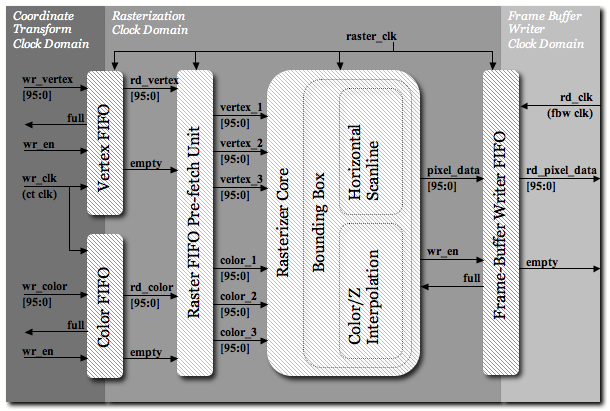
\includegraphics[scale=.80]{raster_high_level.png}
\end{center}
\caption{High-level Diagram of Rasterization Module and Related Interfaces}
\label{fig:buffer_space}
\end{figure}

\subsection{Bounding Box}
\subsection{Horizontal Scanline}
\subsection{Color Interpolation}

\section{Framebuffer/DVI Controller}

\subsection{DVI Controller}
The reference design for the XUPV5 contained a DVI controller that displays a frame buffer on DDR2 SDRAM.  The core outputs a 640 by 480 video over the DVI port of the board.  The core reads a line of the SDRAM frame buffer over the PLB bus and stores it locally in BRAM. Since the frame buffer is any 2MB region in the PLB address space, the frame buffer does not actually have to reside in SDRAM.  Any mapped address can be used as a frame buffer, which demonstrates some of the flexibility of the PLB.  The DVI controller has control registers mapped on the DCR bus interface.  In order for other elements in the system to configure the controller, there is a PLB/DCR bridge what maps the DCR space to a part of the system PLB address space.


\subsection{PLB IPIF}
fbwriter
Using the PLB actually offered great flexibility in the interconnect of cores.  Although it restricted the project in some ways, requiring the use of particular 

\subsection{Frame and Z Buffers}

\begin{figure}[htb]
\begin{center}
%\leavevmode
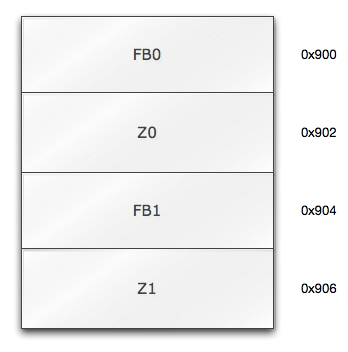
\includegraphics[scale=.68]{buffer_space.png}
\end{center}
\caption{Organization of Buffers}
\label{fig:buffer_space}
\end{figure}

\subsection{DMA}
The DMA module was a late addition to the project.  It is an effort to increase the speed of the flush operation.  Previously, the fbwriter would zero out each pixel individually, requiring far more PLB transactions than necessary.  The fbwriter can program the flush operation to the DMA, which in turn will flush not only the frame buffer but the z-buffer, since they are contiguous in memory.

\section{Development Software}

\subsection{FPGA Tool Chain}
The obvious, and apparently only, choice was Xilinx ISE Design Suite 12.2.  This is not an endorsement, for it is definitely worth the effort to consider an alternative.

\subsubsection{EDK and SDK}
The reference design came as a Platform Studio and Embedded Development Kit (EDK) project.  

OS and Libraries Document Collection and EDK Concept, Tools, and Techniques

\subsubsection{ISE}
We used this to manage multiple hardware projects.  The core had it's own project, which EDK uses to import as a peripheral.  Also, each component 

\subsubsection{CoreGEN}
Another component of the Design Suite used to generate cores.  It was useful in many ways to construct basic hardware elements; see gripes in other sections.

\subsubsection{PlanAhead}
PlanAhead is another component of the Design Suite.  We used it to generate most of our ChipScope modules from netlists.  The netlists comes from the EDK builds and PlanAhead allows us to add ChipScope modules that sample particular signals on real hardware.  It does require a separate bit file and thus, an additional build, but the information is invaluable; this can solve so many of your bugs.  Getting this up early would also yields exponential benefits.

\subsection{Git}
A project without source control is simply unwieldy.  Two group members have had relatively enjoyable experiences with Git, and it was simpler to initialize and set-up than svn, the other likely alternative.  The distributed style allowed for great flexibility moving central repositories and asynchrony of the group's work style.

\subsection{Windows XP}
Operating system that existed on the lab machine and had a licensed installation of the Design Suite was fairly convenient.  Machine was fairly slow, but static ip address and domain name given by the department made it easy to work remotely.

\subsection{Ubuntu}
Initially, wanted machine to be primary machine for development.  Unfortunately, the usb drivers for the JTAG cable never came into fruition, so board programming was relegated to the Windows machine.  Much of the simulation and core development still happened on the Ubuntu box.  Also held a git repository that was later moved to github.  It was used as an easy way to transfer files between group members because Windows networked file system is unusable.  


\section{Major Design Decisions}
\subsection{Floating Point vs. Fixed Point}

\subsection{Synchronization}
With the division of work, and division of operational units of the pipeline, we clearly needed an intuitive, robust mechanism to synchronize the RTL.  fbwriter needs to operate on the PLB bus, so it conformed to the clock of the PLB bus.  Note also that per OpenGG instruction, the rasterization unit has more work than the coordinate transform.  The rasterization unit needs at least one clock cycle for each pixel in the bounding box in the process of horizontal scanline; that means it can vary on the size of the triangle.  The transformation unit has a fixed number of cycles per instruction; it does not vary on the size of the triangle drawn.  Clocking these units independently became extremely convenient.  Using clock independent FIFO's, data can be passed across clock domains safely and efficiently.  The unit will stall only when the queue is full, which is as good as can be expected.

\subsection{External Cores}
It soon became apparent we could not do everything. The decision to conform to the Xilinx tool chain stemmed partially from the convenience of provided Xilinx cores and generated cores from CoreGEN.  The framework provided by the Xilinx EDK had some advantages.  It has a way to run C code a soft processor, the Microblaze.  It provides the interconnecting bus structure, PLB.  The reference design also contains the Multi-Port Memory Controller (MPMC) which provides an accessible interface for the DD2 SDRAM.  

\subsubsection{CoreGEN}
CoreGEN allows us to generate different types of modules.  It is a tool provided by Xilinx included in their design suite and provides blackbox *.v and *.ngc files for usage in your projects.  They provide a variety different, commonly used cores, that is, if it is not a custom type of hardware, you can probably find it in CoreGEN.  Most of the modules in the reference design actually comes from CoreGEN, including the versatile MPMC.  The floating point units used throughout our design were generated to specific parameters.  It was useful to specify usage of DSP48E slices instead of logic slices.  CoreGEN also allowed us to specify latency, which became extremely important.  The FIFO's were also generated by CoreGEN.  It was nice to be able to specify what kind of hardware resources each would consume, whether Block RAM, Distributed RAM or built-in units.  Note that the built-in units may not simulate as easily; simply generate Block RAM modules for simulation and regenerate the cores with the same project file when moving back to synthesis.


\section{Individual Contributions}
\subsection{Andrew Lau}
My primary responsibilities for this project were the implementation of the vertex transformation pipeline and the integration and testing of the various parts of the pipeline. As the only team member who had taken Computer Graphics, much of the graphics design was deferred to me. The first few weeks of the project were spent working closely with Alan to design the front end of the pipeline, specifically how to use GLSim to talk to the pipeline. This idea was quickly squashed as we found that GLSim was deprecated and had not been updated since 2002. The next few weeks were spent designing the ISA, looking for suitable floating point units, investigating alternatives to GLSim, which included Mesa. We ultimately decided to write a primitive Perl script that would parse OpenGL calls and assemble the byte code.

Alan and I worked closely to develop the matrix multiply and matrix stack control modules. These modules implement the 4x4 x 4x4 and 4x4 x 1x4 matrix multiply functionality as well as read in the operands from the correct places. I also wrote the testbenches for these modules, and tested them in simulation to verify correctness.

I was mainly responsible for the coordinate transformation pipeline, as well as the fetch, decode units. The remainder of the semester was spent implementing, testing and integrating this part with the other parts of the pipeline.

\subsection{Alan Zhu}
My responsibilities consisted of implementing the Perl parser, designing and implementing the matrix multiply and matrix stack units, and designing and implementing the rasterizerization module.

At the beginning of the project, I worked closely with Andrew in attempting to us the GLSim frontend to communicate to the pipeline. After a short period of successive failures and finally accepting that the already-broken source code had been sitting in the dust for 8 years, we decided do build everything from the ground up, which would start with implementing our own instruction set that would reflect a primitive version of basic OpenGL commands. 

This also prompted a hunt for critical components that we would need which would be too much overhead to implement (i.e. floating point ALUs), and a search other alternatives to GLSim (which turned up with only huge libraries we didn't have time to deal with). At this time we also had to consider whether we wanted most of the pipeline to work with floating point or fixed point values. Here, the Xilinx tools proved fairly useful, as they included a Core Generator which could generate adders, subtracters, multipliers, and dividers that were all IEEE 32-bit floating point compliant. In hindsight, if proper fixed point arithmetic units could be correctly written and implemented, it would ultimately be best to redesign our project using fixed point inputs, due to the fact there are optimizations limited to fixed point, as well as the fact that the precision offered by floating point is much more than actually necessary.

As our ISA came together, I started putting together the primitive parser that would allow us to write basic programs that the pipeline could understand. Perl seemed like an ideal language not only because of my familiarity with it, but its nature as a scripting language and its excellent manipulation of regular expressions allowed a simple implementation that could potentially make our project a lot less complicated than necessary. Things like converting decimal floating point to binary floating point and calculating sine and cosine values helped us push some of the work to the software side, which would definitely help us focus on the more critical parts of the project. I would find myself adding/modifying the perl script regularly whenever we needed to push some abnormally difficult or confusing functions to the side, most notably calculating and arranging various matrices based on OpenGL specifications.

Much of  Andrew and I then proceeded to design and implement the matrix control modules, namely those for managing the matrix stack and the matrix multiply functions. This was really our big first step into the project, and so we played a lot of our design decisions conservatively (namely, using as little floating point multipliers as necessary). Working together proved useful as we were able to bounce ideas off each other as well as correct one another's logic. Since time wasn't a luxury, after the basic matrix functionality was completed, Andrew took onthe rest of the coordinate transform pipeline, including more complicated testing procedures with our baseline implementation, and I moved on to other necessary components, namely the rasterizer.

The other bulk of my efforts went in to designing the rasterization unit. The rasterization unit proved to be fairly intuitive to implement, and in hindsight, not overly complicated nor difficult if the high-level idea is clear. I actually thought the harder part included interfacing the rasterizer with the coordinate transform FIFO. Since coordinate transform and rasterization are done in separate clock comains, the state machine that controls the timing is everything. The acutal raster calculations were very easy to debut and pretty much worked after one or two edits to the first draft of the code. 

One thing I really regret about this portion of the project is that we decided to use combinational logic, and did not pipeline the rasterizer from the very beginning. The group was pressed for time near the end of the project, so our focus was more on getting the entire system to work, rather than tuning performance without guaranteeing correctness. In hindsight, the straightforward combinational approach makes implementation much simpler and eaiser to understand, but at a substantial cost in performance.  

The Xilinx Core Generator can generate floating point units with user-specified latency so combined with a fixed-point pipeline implementation, the rasterizer (normally considered the computational bottleneck) has significant potential for high performance. Of course, the caveat here is that much more logic is required due to the increased control inherent in pipelining and added latency. Also, some optimizations can be achieved simply by having more floating point multipliers and dividers available.

Nevertheless, our rasterizer performed significantly well considering we added little optimization into the design. In fact, it's likely that in the end the rasterizer may not have been the bottleneck, since we also made many design sacrifices in the other components to balance resource utilization. In general, our project was a success, in the sense that any improvements we could have made would mostly be bells and whistles. 

As far as contributions go, we all took on separate responsibilities at certain points in the project, and I feel like the work distribution was extremely well balanced. Having been good friends prior to the class, our team dynamic proved invaluable later on. Although we did not know every intricate detail of what each person was doing, we were always able to just bounce design and implementation decisions off one another, as well as occasionally help one another debug. Working together at the same times in lab also helped set aside dedicated time to work on the project. Of course, being ambitious seniors we all had significant coursework outside of the class which taxed our project noticeably.

I was quite motivated after seeing decently successful results of our project to pipeline the rasterizer but given the amount of work I had in other courses after the final demonstration, I was not able to fully implement a pipelined rasterizer. Another part of the rationale was that it probably isn't the current bottleneck in our project. The code repository includes a semi-completed version of the rasterizer and corresponding FIFO management unit that I began to pipeline at the end of our project, but was not able to complete.
\subsection{Nathan Wan}

My main responsibilities involved the interfaces for the pipeline and the tool set.

One Man Tools Team

Webserver/SDK work

I was mainly in charge of any software that ran on the Microblaze processor.  When we were considering a web-server front-end for our accelerator, I was working with the lwip library on the SDK trying to get the webserver running.  The current design uses an assembler to get data from Perl Parser to the pipeline.

As the build engineer, I was left with most of the decisions on the system level.   

On the final day, with pressure to bring down EDK utilization, I took SRAM out of the project.  Unbeknownst to me, SRAM actually contained configuration data necessary for the Microblaze to run.  That left us with a broken build pretty close to demo time.   The lesson here is to ensure you know exactly what you're cutting out of the reference design, or know as much as possible.

\section{Status and Future Work}

\subsection{Tool Chain}
If I recall correctly, no guidance on the Xilinx Design Suite because we were encouraged to look for alternatives.  That is, we were not to be restricted to Xilinx tools.  Yet, no alternatives were found, none were found by other classmates.  Getting a tool chain or build process up early is a huge key to success.  This should be a priority for every group. 	

\subsection{CPU Integration}
Use Instruction Cache as a ring buffer for instructions.  Interrupt Microblaze every time the cache is consumed.

\subsection{Shader}
A very interesting project would be to work on a graphics shader.  OpenGL ES 2.0 relies primary on the shader to replace many fixed function units in the pipeline.  Although most of those units are effect units, and unimplemented in our implementation, the project would be interesting as it is the main unit in GPGPU Frameworks.  It also requires a microkernel to run in hardware, which would make for a interesting fusion of OS and hardware.

\subsection{MPMC}
DMA, P2P PLB, PLB alternative

\subsection{vsync Timing}

\section{Class Impression/Improvements}

\subsection{Tool Chain Frustration}
\subsection{Too much Independence / Lack of Feedback}

\section{Citations}

% Xilinx manuals

\section{Credits}

% Prof and course staff

% Ken Mai for initial meeting

% Google Docs

% OpenGG Tumblr

% LaTeX and diagramming program

\end{document}